%copyright 2007 by Till Tantau
%
% This file may be distributed and/or modified
%
% 1. under the LaTeX Project Public License and/or
% 2. under the GNU Public License.
%
% See the file doc/licenses/LICENSE for more details.



\documentclass{beamer}

%
% DO NOT USE THIS FILE AS A TEMPLATE FOR YOUR OWN TALKS¡!!
%
% Use a file in the directory solutions instead.
% They are much better suited.
%


% Setup appearance:

\usetheme{Darmstadt}
\usefonttheme[onlylarge]{structurebold}
\setbeamerfont*{frametitle}{size=\normalsize,series=\bfseries}
\setbeamertemplate{navigation symbols}{}


% Standard packages

\usepackage[english]{babel}
\usepackage[latin1]{inputenc}
\usepackage{times}
\usepackage[T1]{fontenc}


% Setup TikZ

\usepackage{tikz}
\usetikzlibrary{arrows}
\usetikzlibrary{calc}
\usepackage{pgfmath}
\tikzstyle{block}=[draw opacity=0.7,line width=1.4cm]


% Author, Title, etc.

\title[Monitor Platform Architecture Specs] 
{%
Monitor Platform Architecture Spec %
}

\author[Sinha N]
{
  Nish~Sinha\inst{1} \and
}

\institute[Xad]
{
  \inst{1}%
  Xad Inc., Mountain View, USA
  \and
  \vskip-2mm
}

\date[\today]
{\today}



% The main document

\newcommand{\drawLinkArrow}[4]{
		\pgfmathparse{2pt+3.5pt}
	%\draw[->] let
		%\p1 = ($(#1)), \p2 = ($(#2)),
		%\p3 = ($(#3)), \p4 = ($(#4)) 
		%in ($ (\x1 + \x2)*1/2$ ,\y1) -| ($ (\x3 + \x4)*1/2$ ,\y4);
	\draw[->] let
		\p1 = (#1), \p2 = (#2),
		\p3 = (#3), \p4 = (#4)
		in
		({(\x1 + \x2)*1/2} ,\y1) -- ({(\x3 + \x4)*1/2} ,\y4);
}

%\draw (A) let
%\p1 = ($ (B) - (A) $)
%\n1 = ($ 1 $)
%in
%circle ({veclen(\x1,\y1)});

\begin{document}

\begin{frame}
  \titlepage
\end{frame}

\begin{frame}{Outline}
  \tableofcontents
\end{frame}


\section{Introduction}

\subsection{The Architecture}

\begin{frame}{Diagram}
   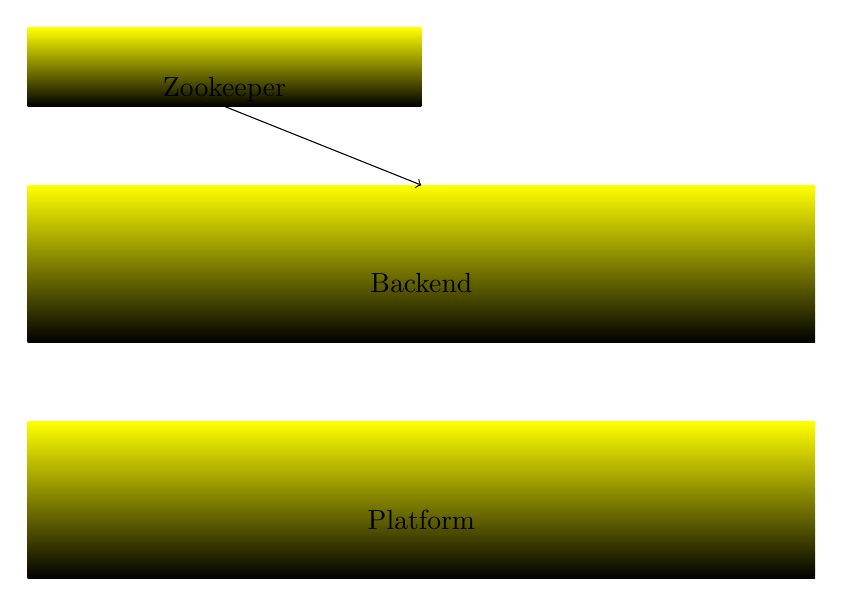
\begin{tikzpicture}
     
	\coordinate (B1_L) at (0,0);
	\coordinate (B1_R) at (5,1);
	\coordinate (B2_L) at (0,-3);
	\coordinate (B2_R) at (10,-1);
	\coordinate (B3_L) at (0,-6);
	\coordinate (B3_R) at (10,-4);
   	\shade[top color=yellow,bottom color=black] (B1_L) rectangle (B1_R) node[midway,below] {Zookeeper};
   	\shade[top color=yellow,bottom color=black] (B2_L) rectangle (B2_R) node[midway,below] {Backend};
   	\shade[top color=yellow,bottom color=black] (B3_L) rectangle (B3_R) node[midway,below] {Platform};
	\drawLinkArrow{B1_L}{B1_R}{B2_L}{B2_R}


  \end{tikzpicture}

\end{frame}




%\begin{frame}[t]{General formalization of haplotyping.}
%  \begin{block}{Inputs}
%    \begin{itemize}
%    \item A \alert{genotype matrix} $G$.
%    \item The \alert{rows} of the matrix are \alert{taxa / individuals}.
%   \item The \alert{columns} of the matrix are \alert{SNP sites /
%       characters}. 
%  \end{itemize}
% \end{block}
 %  \begin{block}{Outputs}
 %    \begin{itemize}
 %    \item A \alert{haplotype matrix} $H$.
 %    \item Pairs of rows in $H$ \alert{explain} the rows of $G$.
 %    \item The haplotypes in $H$ are \alert{biologically plausible}. 
%    \item<alert{Data missing}->
      The problem is directed: one haplotype is known.
 %    \end{itemize}
 %  \end{block}
%  \begin{enumerate}
%  \end{enumerate}
% \end{frame}



\subsection{The Integrated Approach}

\begin{frame}{How blocks help in perfect phylogeny haplotyping.}
  \begin{enumerate}
  \item Partition the site set into overlapping contiguous blocks.
  \item Compute a perfect phylogeny for each block and combine them.
  \item Use dynamic programming for finding the partition.
  \end{enumerate}

  \begin{tikzpicture}
    \useasboundingbox (0,-1) rectangle (10,2);
    
    \draw[line width=4mm,dash pattern=on 3mm off 1mm]
      (0,1) -- (9.99,1) node[midway,above] {Genotype matrix}
      (0,0) -- (9.99,0) node[midway,below] {\only<1>{no perfect phylogeny}};

    \begin{scope}[xshift=-.5mm]
      \only<2->
      {
        \draw[red,block]            (0,.5)   -- (3,.5)
          node[midway,below] {perfect phylogeny};
      }
    \end{scope}
  \end{tikzpicture}
\end{frame}



\section{Bad News: Hardness Results}

\subsection{Hardness of PP-Partitioning of Haplotype Matrices}

\begin{frame}{Finding pp-partitions of haplotype matrices.}
  \begin{example}
    \begin{columns}
      \column{.3\textwidth}
      $M\colon$
      \footnotesize
      \begin{tabular}{cccc}
        0 & 0 & 0 & 1 \\
        0 & 1 & 0 & 0 \\
        1 & 0 & 0 & 0 \\
        0 & 1 & 0 & 0 \\
        1 & 0 & 0 & 0 \\
        0 & 1 & 0 & 1 \\
        1 & 1 & 0 & 0 \\
        0 & 0 & 1 & 0 \\
        1 & 0 & 1 & 0
      \end{tabular}%
      \only<2>
      {%
        
\begin{tikzpicture}
          \useasboundingbox (2.9,0);

          \draw [red, opacity=0.7,line width=1cm] (1.7 ,1.9) -- (1.7 ,-1.7);
          \draw [blue,opacity=0.7,line width=5mm] (0.85,1.9) -- (0.85,-1.7)
                                                  (2.55,1.9) -- (2.55,-1.7);
        \end{tikzpicture}
      }
      \column{.6\textwidth}
      \begin{overprint}
        \onslide<1>
        No perfect phylogeny is possible.
        
        \onslide<2>
        \textcolor{blue!70!bg}{Perfect phylogeny}
        
        \textcolor{red!70!bg}{Perfect phylogeny}
        
        $\chi_{\operatorname{PP}}(M) = 2$.
        
      \end{overprint}
    \end{columns}
  \end{example}
\end{frame}

\subsection{Hardness of PP-Partitioning of Genotype Matrices}


\begin{frame}{Finding pp-partitions of genotype matrices.}
  Now comes the general case:
  \begin{itemize}
  \item The inputs $M$ are \alert{genotype matrices}.
  \item The inputs $M$ \alert{do not allow a perfect phylogeny}.
  \item What is $\chi_{\operatorname{PP}}(M)$?
  \end{itemize}
  \begin{example}
    \begin{columns}
      \column{.3\textwidth}
      $M\colon$
      \footnotesize
      \begin{tabular}{cccc}
        2 & 2 & 2 & 2 \\
        1 & 0 & 0 & 0 \\
        0 & 0 & 0 & 1 \\
        0 & 0 & 1 & 0 \\
        0 & 2 & 2 & 0 \\
        1 & 1 & 0 & 0 
      \end{tabular}%
      \only<2>
      {%
        
\begin{tikzpicture}
          \useasboundingbox (2.9,0);
          
          \draw [red, opacity=0.7,line width=1cm] (1.7 ,1.3) -- (1.7 ,-1.1);
          \draw [blue,opacity=0.7,line width=5mm] (0.85,1.3) -- (0.85,-1.1)
                                                  (2.55,1.3) -- (2.55,-1.1);
        \end{tikzpicture}
      }
      \column{.6\textwidth}
      \begin{overprint}
        \onslide<1>
        No perfect phylogeny is possible.
        
        \onslide<2>
        \textcolor{blue!70!bg}{Perfect phylogeny}
        
        \textcolor{red!70!bg}{Perfect phylogeny}
        
        $\chi_{\operatorname{PP}}(M) = 2$.
        
      \end{overprint}
    \end{columns}
  \end{example}
\end{frame}





\section{Good News: Tractability Results}

\subsection{Perfect Path Phylogenies}



\begin{frame}{Example of a perfect path phylogeny.}
  \begin{columns}[t]
    \column{.3\textwidth}
    \begin{exampleblock}{Genotype matrix}
      $G\colon$
      \begin{tabular}{ccc}
        A & B & C \\\hline
        2 & 2 & 2 \\
        0 & 2 & 0 \\
        2 & 0 & 0 \\
        0 & 2 & 2 
      \end{tabular}
    \end{exampleblock}

    \column{.3\textwidth}
    \begin{exampleblock}{Haplotype matrix}
      $H\colon$
      \begin{tabular}{ccc}
        A & B & C \\\hline
        1 & 0 & 0 \\
        0 & 1 & 1 \\
        0 & 0 & 0 \\
        0 & 1 & 0 \\
        0 & 0 & 0 \\
        1 & 0 & 0 \\
        0 & 0 & 0 \\
        0 & 1 & 1 
      \end{tabular}
    \end{exampleblock}

    \column{.4\textwidth}
    \begin{exampleblock}{Perfect path phylogeny}
      \begin{center}
        \begin{tikzpicture}[auto,thick]
          \tikzstyle{node}=%
          [%
            minimum size=10pt,%
            inner sep=0pt,%
            outer sep=0pt,%
            ball color=example text.fg,%
            circle%
          ]
        
          \node [node] {} [->]
            child {node [node] {} edge from parent node[swap]{A}}
            child {node [node] {}
              child {node [node] {} edge from parent node{C}}
              edge from parent node{B}
            };
        \end{tikzpicture}
      \end{center}
    \end{exampleblock}
  \end{columns}
\end{frame}



\subsection{Tractability of PPP-Partitioning of Genotype Matrices}


\appendix

\section*{Appendix}


\end{document}

